\section{Question 8 : Critère de bascule orienté réseau (décision côté PGW)}
% ---------------------------------------------------------------------

\subsection{Objectif}
Les questions précédentes étudient un critère \emph{orienté terminal} : c'est
l'UE qui mesure sa distance (ou son RSSI) et qui modifie sa table de routage.
La question B8 implémente l'approche duale, inspirée des architectures
d'offloading pilotées par le c\oe ur de réseau (PGW/ANDSF) : la décision est
prise \emph{par flux applicatif}, selon le protocole de transport et le débit,
indépendamment de la position de l'UE.

\subsection{Principe de décision}
NS-3 ne modélise ni l'ANDSF ni le PCRF. Le rôle du PGW est donc simulé par une
fonction exécutée \emph{une seule fois par flux}, avant le démarrage du trafic.
La règle appliquée est celle de l'énoncé :
\[
\text{Wi-Fi} \iff (\text{protocole} = \text{UDP}) \;\wedge\; (D_{\text{flux}} > D_{\text{seuil}}),
\qquad D_{\text{seuil}} = 1~\text{Mb/s},
\]
et LTE dans tous les autres cas. Ainsi, un flux UDP à débit élevé est déchargé
vers le Wi-Fi, tandis qu'un flux TCP reste sur LTE, où l'EPC garantit
l'ordonnancement et la qualité de service.

\begin{lstlisting}[language=C++]
static bool PolicyOffloadToWifi(bool isUdp, double rateMbps, double thrMbps)
{
    return isUdp && rateMbps > thrMbps;   // UDP au-dessus du seuil -> Wi-Fi
}
\end{lstlisting}

\begin{figure}[H]
      \centering
      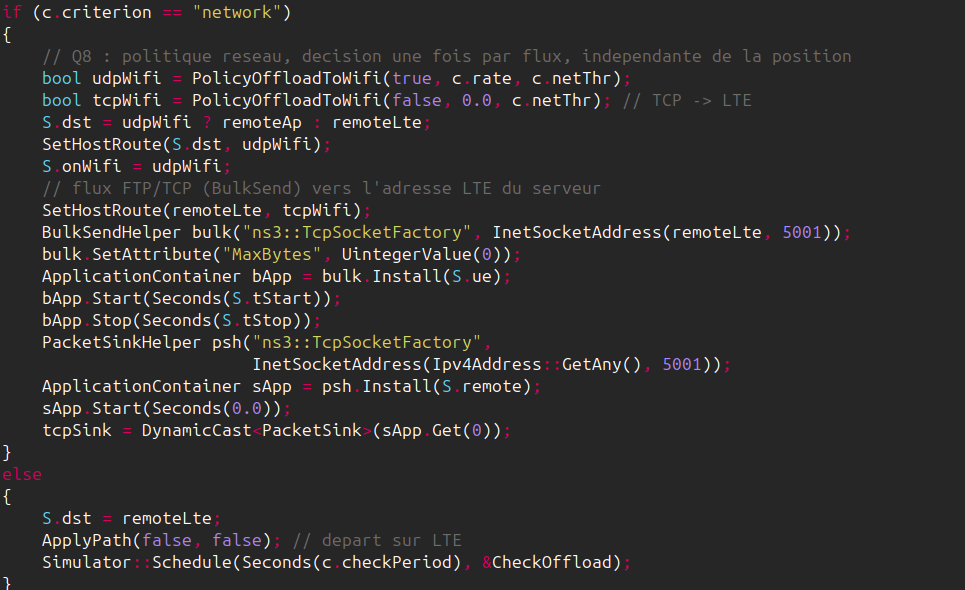
\includegraphics[width=0.7\textwidth]{img/C/pic0_criterion.png}
      \caption{Capture de la Configuration des modes }
\end{figure}

\subsection{Scénario et paramètres}
Le scénario de la question B1 est repris (un eNodeB, un point d'accès Wi-Fi
802.11n, un UE à double interface, un serveur distant). Deux flux
\emph{simultanés} sont émis de l'UE vers le serveur (sens montant) :

\begin{itemize}
  \item un flux \textbf{UDP CBR} de 2~Mb/s (paquets de 1200 octets, port 9000),
        supérieur au seuil de 1~Mb/s : il est donc routé vers le Wi-Fi ;
  \item un flux \textbf{TCP} de type FTP (\texttt{BulkSendApplication}, port
        5001), routé vers LTE.
\end{itemize}

Le routage est réalisé par des routes \emph{hôte} statiques
(\texttt{AddHostRouteTo}) dans la table de l'UE : le flux UDP est adressé à
l'adresse Wi-Fi du serveur (10.0.2.2, joignable via l'AP), le flux TCP à son
adresse LTE (1.0.0.2, joignable via le PGW). Ces routes ne sont jamais
modifiées pendant la simulation.

\begin{table}[H]
\centering
\caption{Adressage et chemins utilisés dans la question B8}
\begin{tabular}{llll}
\toprule
Flux & Source & Destination & Chemin \\
\midrule
UDP CBR 2 Mb/s (port 9000) & 10.0.1.2 (UE, Wi-Fi) & 10.0.2.2 (serveur) & UE $\to$ AP $\to$ serveur \\
TCP bulk (port 5001)       & 7.0.0.2 (UE, LTE)    & 1.0.0.2 (serveur) & UE $\to$ eNodeB $\to$ PGW $\to$ serveur \\
\bottomrule
\end{tabular}
\end{table}

\begin{lstlisting}
                     +---- LTE path ------------------------------+
                     |                                             |
UE --(LTE radio)--> eNodeB --(S1)--> SGW/PGW --(p2p 1.0.0.0/8)--> RemoteHost
 |                                                                   ^
 +--(WiFi radio)--> AP --------(p2p 10.0.2.0/24)---------------------+
                     +---- WiFi path ----+
\end{lstlisting}

\subsection{Vérification par FlowMonitor et pcap}
La vérification a été effectuée sur une exécution de contrôle où l'UE démarre
dans la zone du hotspot (vitesse 1~m/s, durée 20~s), afin que les premiers
paquets du flux UDP puissent effectivement traverser le Wi-Fi :
\begin{lstlisting}
./ns3 run "tp3-offload --criterion=network --speed=1 --simTime=20 \
           --pcap=true --outDir=results/tp3/q8 --tag=net_proof"
\end{lstlisting}

Le fichier de synthèse de cette exécution donne : 4\,500\,000 octets émis sur
le chemin Wi-Fi et 4\,500\,000 octets reçus par le serveur via le Wi-Fi, aucune
perte, un débit moyen de 2,00~Mb/s pour le flux UDP et un débit de
1,65~Mb/s pour le flux TCP (via LTE). Aucune bascule n'est comptabilisée,
conformément au principe du critère réseau.

\begin{figure}[H]
      \centering
      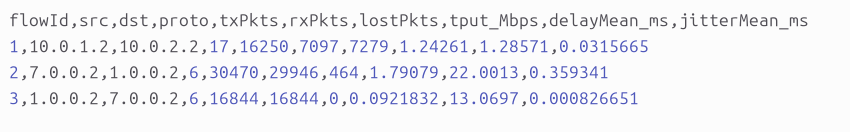
\includegraphics[width=0.7\textwidth]{img/C/pic1_flowmon.png}
      \caption{Deux flux : UDP 10.0.1.2 $\to$ 10.0.2.2 et TCP 7.0.0.2 $\to$ 1.0.0.2}
\end{figure}


\paragraph{Capture Wireshark.}
Les captures pcap sont ouvertes dans Wireshark :
\begin{itemize}
  \item sur la liaison AP--serveur (\texttt{*\_remote-ap*.pcap}), avec le filtre
        \texttt{udp.port == 9000}, on observe le flux UDP dès son premier
        paquet ; aucun segment TCP n'y figure ;
  \item sur la liaison PGW--serveur (\texttt{*\_remote-lte*.pcap}), avec le
        filtre \texttt{tcp.port == 5001}, on observe le flux TCP, et
        \emph{aucun} paquet UDP de port 9000.
\end{itemize}

\begin{figure}[H]
      \centering
      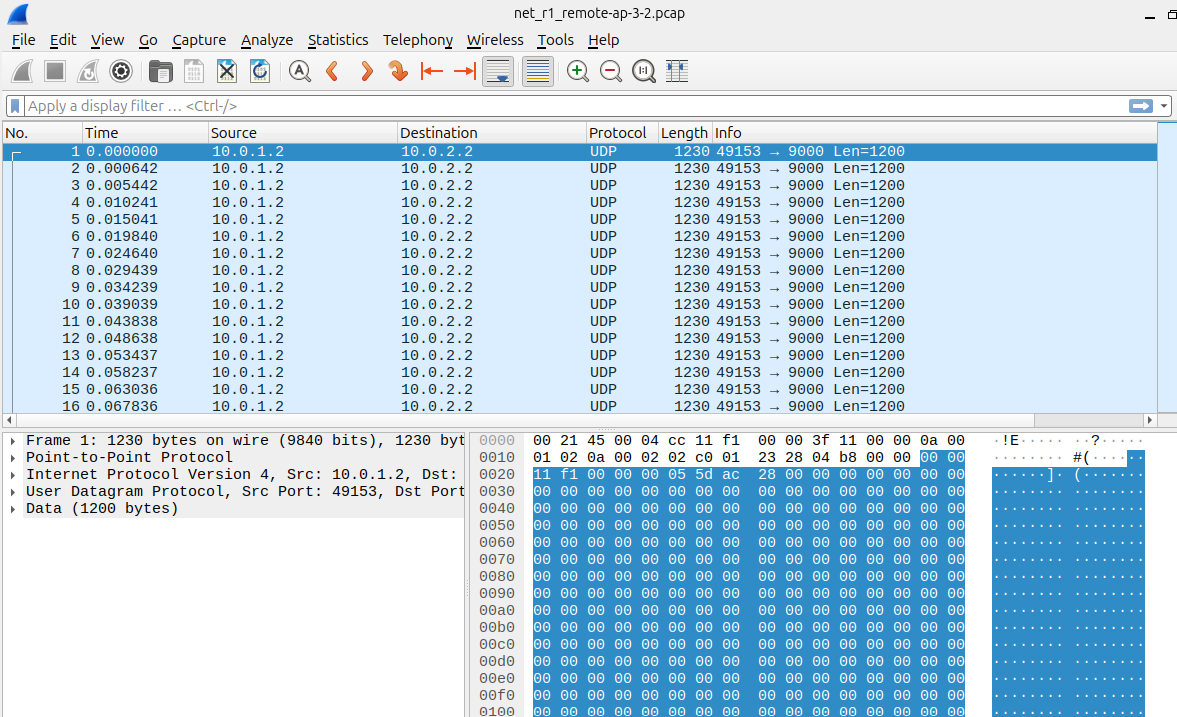
\includegraphics[width=0.7\textwidth]{img/C/pic2_udp_flow.png}
      \caption{flux des paquets UDP de l'adresse source 10.0.1.2}
\end{figure}

\begin{figure}[H]
      \centering
      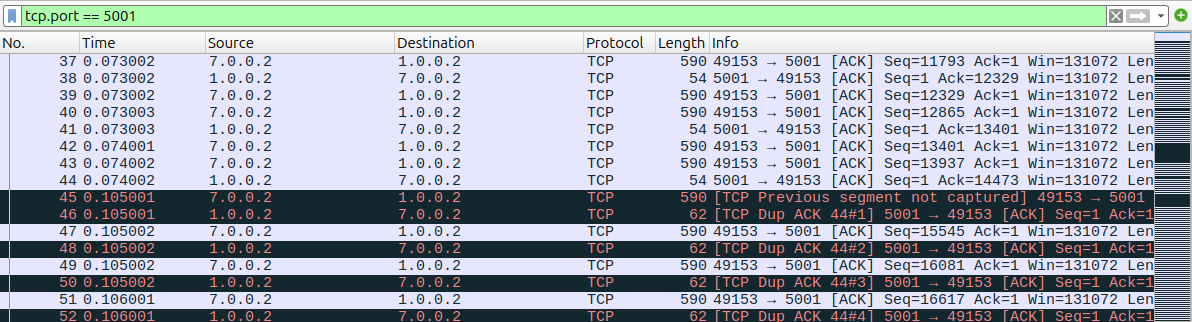
\includegraphics[width=0.7\textwidth]{img/C/pic3_tcp.png}
      \caption{le handshake TCP SYN/SYN-ACK dès t $\approx$ 1 s et l'absence de trafic UDP 9000}
\end{figure}

\subsection{Limites de la modélisation}
\begin{itemize}
  \item La fonction de politique est exécutée dans la simulation et agit sur la
        table de routage de l'UE : le PGW n'est pas une entité décisionnelle
        distincte, conformément à la simplification demandée par l'énoncé.
  \item La décision est statique : elle est prise au démarrage de chaque flux
        et n'est pas réévaluée en cours de route.
  \item Les flux sont émis dans le sens montant ; en sens descendant, le choix
        du chemin relèverait de la table de routage du serveur.
\end{itemize}

\subsection{Conclusion de B8}
La politique orientée réseau fonctionne comme attendu : le flux UDP à 2~Mb/s
emprunte le Wi-Fi dès son premier paquet et le flux TCP reste sur LTE, ce qui
est confirmé par FlowMonitor et par les captures pcap. Le comportement de ce
critère en situation de mobilité est étudié à la question B9.

% ---------------------------------------------------------------------
\section{Question 9 : Comparaison des critères orienté terminal et orienté réseau}
% ---------------------------------------------------------------------

\subsection{Protocole expérimental}
Les trois configurations suivantes sont comparées sur la \emph{même
trajectoire} et les \emph{mêmes graines} :
\begin{itemize}
  \item \texttt{dist\_h0} : critère terminal à seuil de distance unique ($H=0$) ;
  \item \texttt{dist\_h5} : critère terminal avec hystérésis ($H=5$~m, seuils
        d'entrée et de sortie à 45~m et 55~m) ;
  \item \texttt{net} : critère réseau de la question B8.
\end{itemize}

\begin{table}[H]
\centering
\caption{Paramètres de la campagne de la question B9}
\begin{tabular}{ll}
\toprule
Paramètre & Valeur \\
\midrule
Rayon nominal du hotspot $R$ & 50 m \\
Trajectoire & ligne droite traversant l'AP (\texttt{line}) \\
Vitesse de l'UE & 5 m/s \\
Durée de simulation & 80 s (trafic de 1 s à 79 s) \\
Débit CBR UDP & 2 Mb/s (paquets de 1200 octets) \\
Décalage latéral aléatoire & $b \sim \mathcal{U}(0,\,0{,}5\,R)$ (\texttt{offsetFrac}=0,5) \\
Bruit de mesure de distance (critères terminal) & $\sigma_d = 3$ m (\texttt{distNoise}=3) \\
Shadowing & désactivé (\texttt{shadowSigma}=0) \\
Période de vérification du critère & 0,5 s \\
Fenêtre de détection du ping-pong & 15 s (valeur par défaut du code) \\
Graine / numéros de run & graine = 1 / runs 1 à 5 \\
Nombre de simulations & $3 \times 5 = 15$ \\
\bottomrule
\end{tabular}
\end{table}

Le décalage latéral $b$ est tiré avec la même graine pour les trois
configurations : à numéro de run égal, les trois critères parcourent donc
exactement la même trajectoire (valeur de \texttt{offset\_b} identique dans
les fichiers de synthèse). Les moyennes sont accompagnées de l'écart-type
expérimental (correction de Bessel).

\paragraph{Définition de l'interruption.}
La définition de la question B4 est reprise : une interruption est une durée
pendant laquelle le débit reçu tombe sous 50\,\% du débit nominal. Dans cette
campagne, elle est évaluée sur des intervalles \emph{fixes} de 100~ms (et non
sur une fenêtre glissante) autour de chaque bascule, avec le nombre de
paquets perdus et le pic de délai sur cette fenêtre. La résolution temporelle
est donc de 100~ms. Pour le critère réseau, aucune bascule n'a lieu en cours
de flux : l'interruption \emph{par bascule} est sans objet (N/A).

\subsection{Résultats}

\begin{table}[H]
\centering
\caption{Commutations, offloading et interruption (moyenne $\pm$ écart-type sur 5 runs)}
\small
\begin{tabular}{lccccc}
\toprule
Config. & Bascules & Ping-pong & Offloading & Interruption & Pic de délai \\
        &          &           & effectif$^{(a)}$ & par bascule (s) & (ms) \\
\midrule
\texttt{dist\_h0} & $3{,}20 \pm 1{,}10$ & $1{,}20 \pm 1{,}10$ & $0{,}24 \pm 0{,}01$ & $0{,}00 \pm 0{,}00$ & $21{,}07 \pm 2{,}20$ \\
\texttt{dist\_h5} & $2{,}00 \pm 0{,}00$ & $0{,}00 \pm 0{,}00$ & $0{,}25 \pm 0{,}02$ & $0{,}00 \pm 0{,}00$ & $20{,}23 \pm 2{,}43$ \\
\texttt{net}      & $0{,}00 \pm 0{,}00$ & $0{,}00 \pm 0{,}00$ & $\approx 0{,}43$ $^{(b)}$ & N/A & N/A \\
\bottomrule
\end{tabular}

\smallskip
\begin{minipage}{0.92\textwidth}\footnotesize
$^{(a)}$ Fraction des octets \emph{reçus par le serveur via le Wi-Fi}.\\
$^{(b)}$ Le fichier de synthèse affiche 1,00 pour \texttt{net}, car seuls les
octets \emph{reçus} sont comptés et tous sont passés par le Wi-Fi. Rapporté au
volume \emph{émis}, l'offloading effectif vaut $1 - 0{,}5704 \approx 0{,}43$.
(sur le run 1, des paquets sont encore reçus via le Wi-Fi jusqu'à
85,5~m de l'AP, soit un rayon effectif d'environ 85~m).
\end{minipage}
\end{table}

\begin{table}[H]
\centering
\caption{Qualité de service (moyenne $\pm$ écart-type sur 5 runs)}
\small
\begin{tabular}{lcccc}
\toprule
Config. & Perte (\%) & Délai moyen (ms) & Durée sous le seuil (s) & Débit moyen (Mb/s) \\
\midrule
\texttt{dist\_h0} & $0{,}00 \pm 0{,}00$ & $13{,}58 \pm 0{,}20$ & $0{,}00 \pm 0{,}00$ & $2{,}00 \pm 0{,}00$ \\
\texttt{dist\_h5} & $0{,}00 \pm 0{,}00$ & $13{,}52 \pm 0{,}28$ & $0{,}00 \pm 0{,}00$ & $2{,}00 \pm 0{,}00$ \\
\texttt{net}      & $57{,}04 \pm 0{,}59$ & $1{,}29 \pm 0{,}01$ & $44{,}48 \pm 0{,}44$ & $0{,}86 \pm 0{,}01$ \\
\bottomrule
\end{tabular}

\smallskip
\begin{minipage}{0.92\textwidth}\footnotesize
La durée sous le seuil est cumulée sur toute la simulation (sur 78 s de
trafic), et non par bascule. Le délai moyen de \texttt{net} ne porte que sur
les paquets effectivement livrés, tous par le Wi-Fi.
\end{minipage}
\end{table}

\begin{figure}[H]
      \centering
      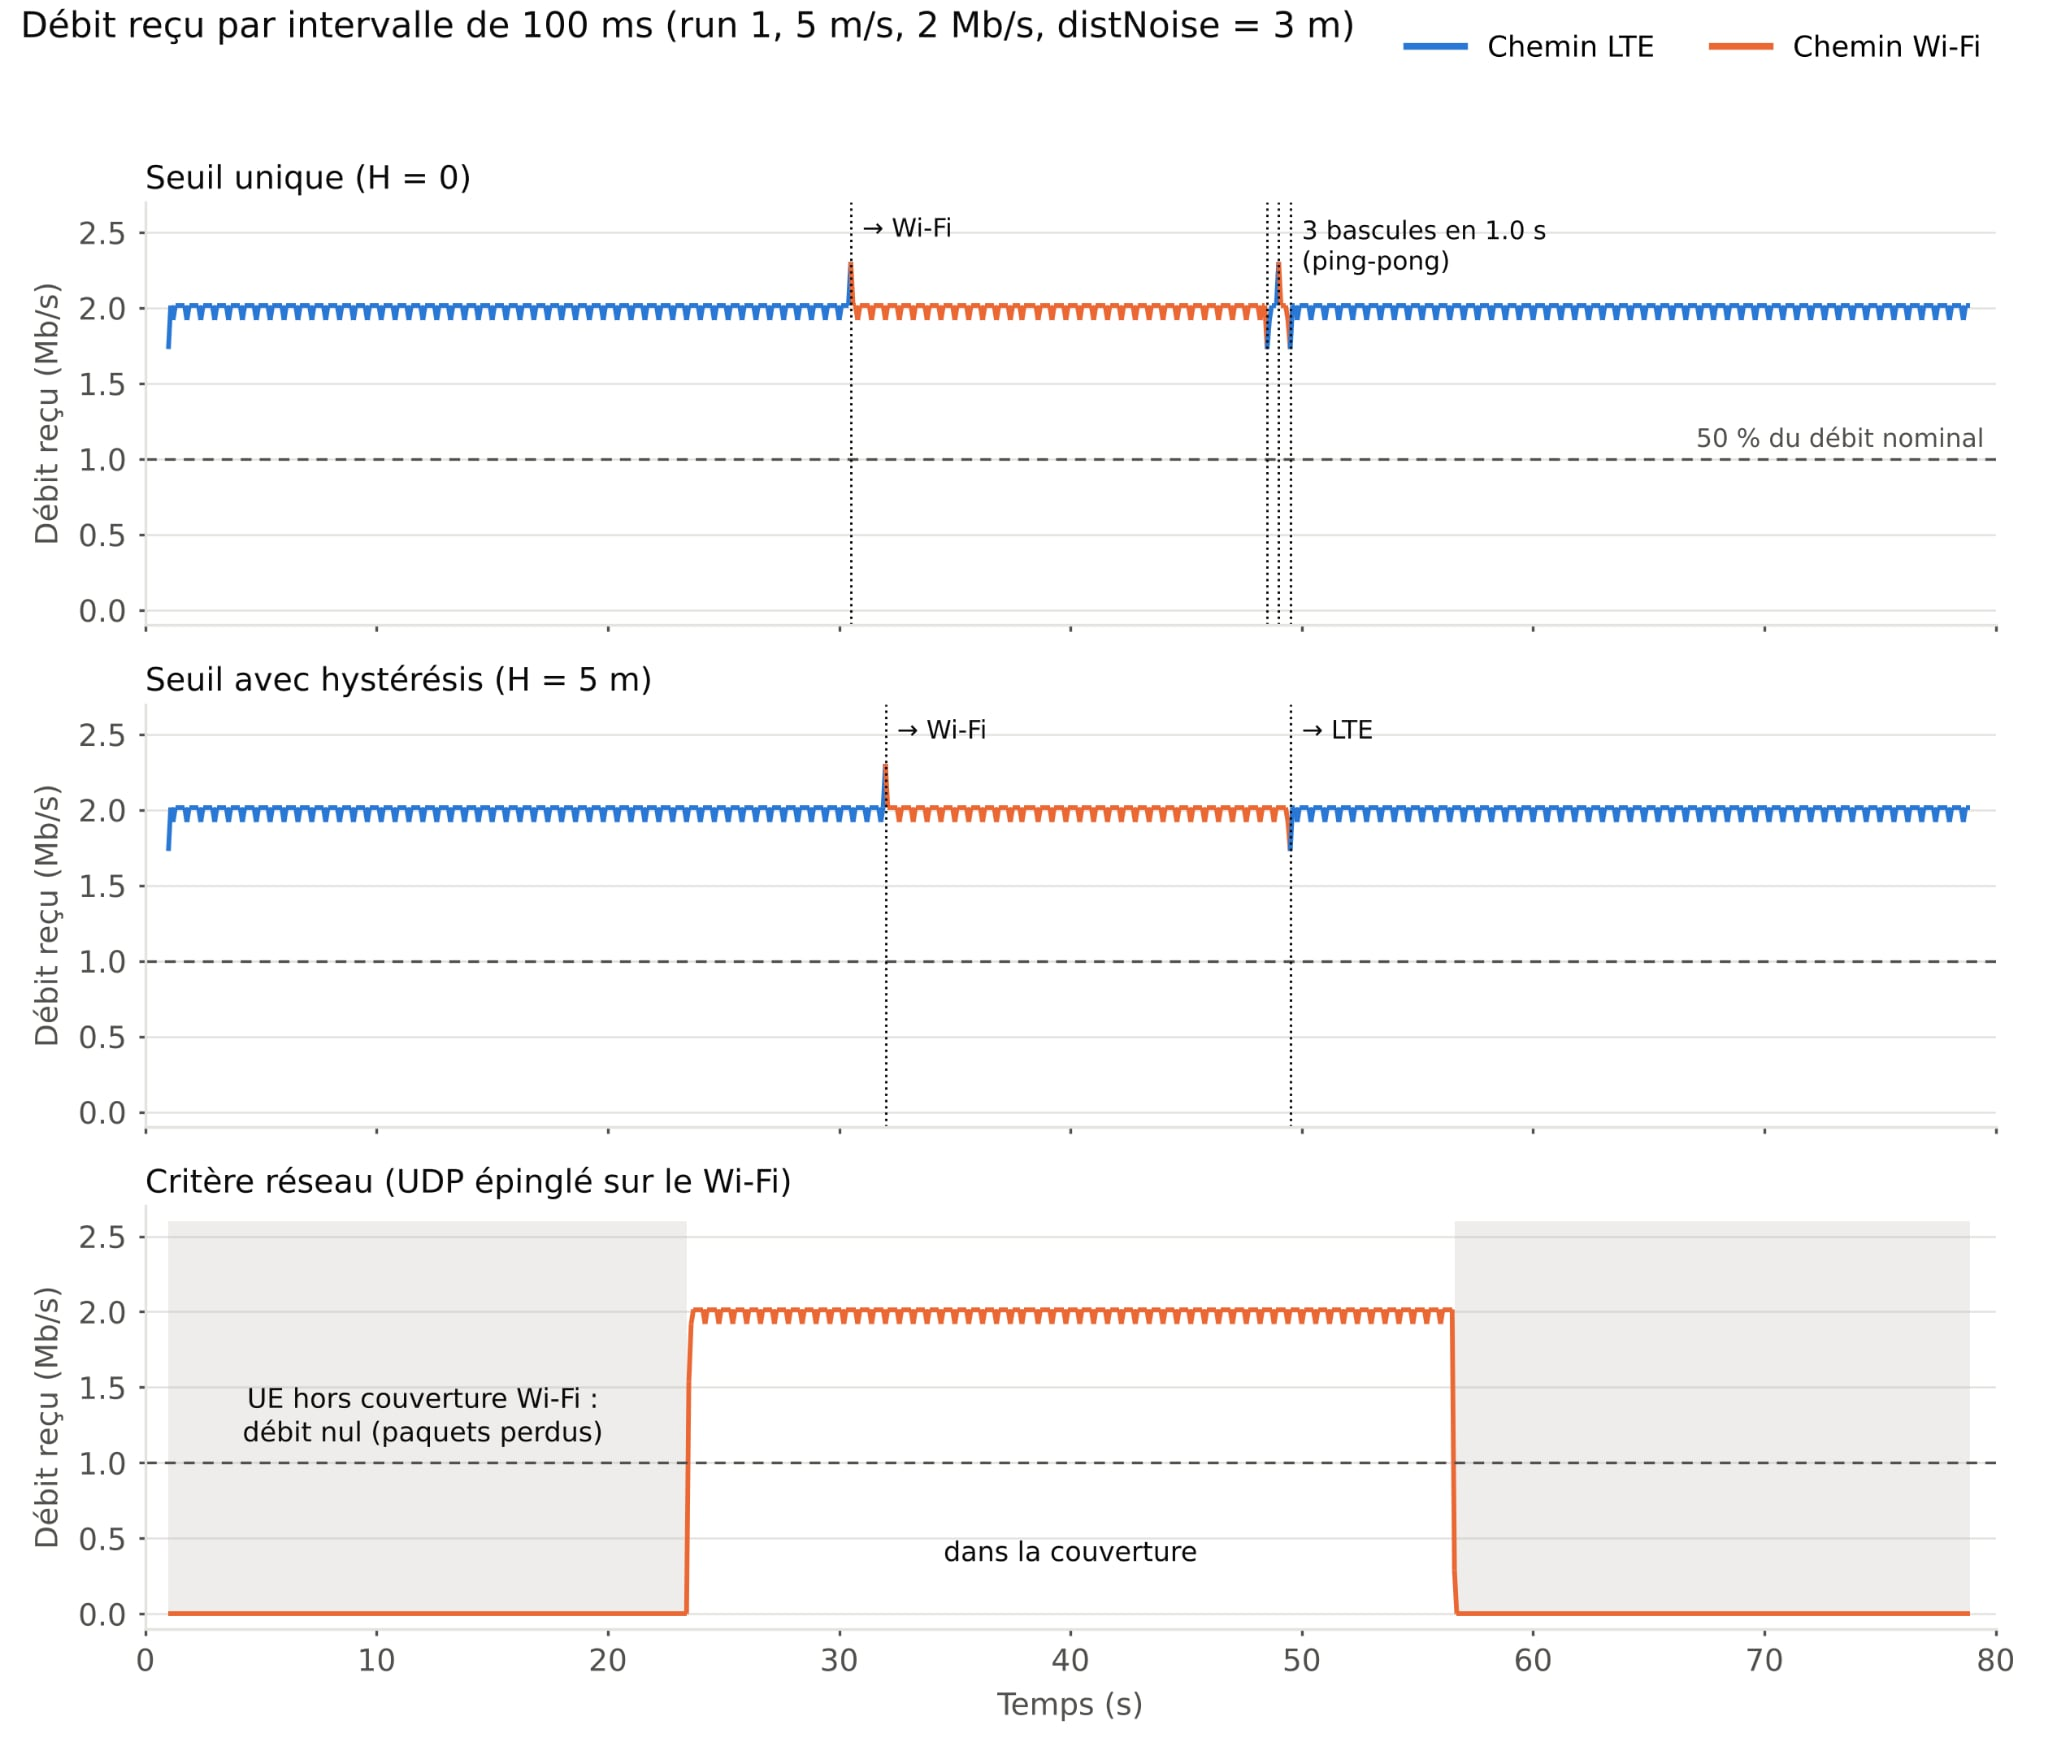
\includegraphics[width=0.7\textwidth]{img/C/pic4_debitudp.jpg}
      \caption{Nombre de bascules et taux d'offloading par critère}
\end{figure}
\begin{figure}[H]
      \centering
      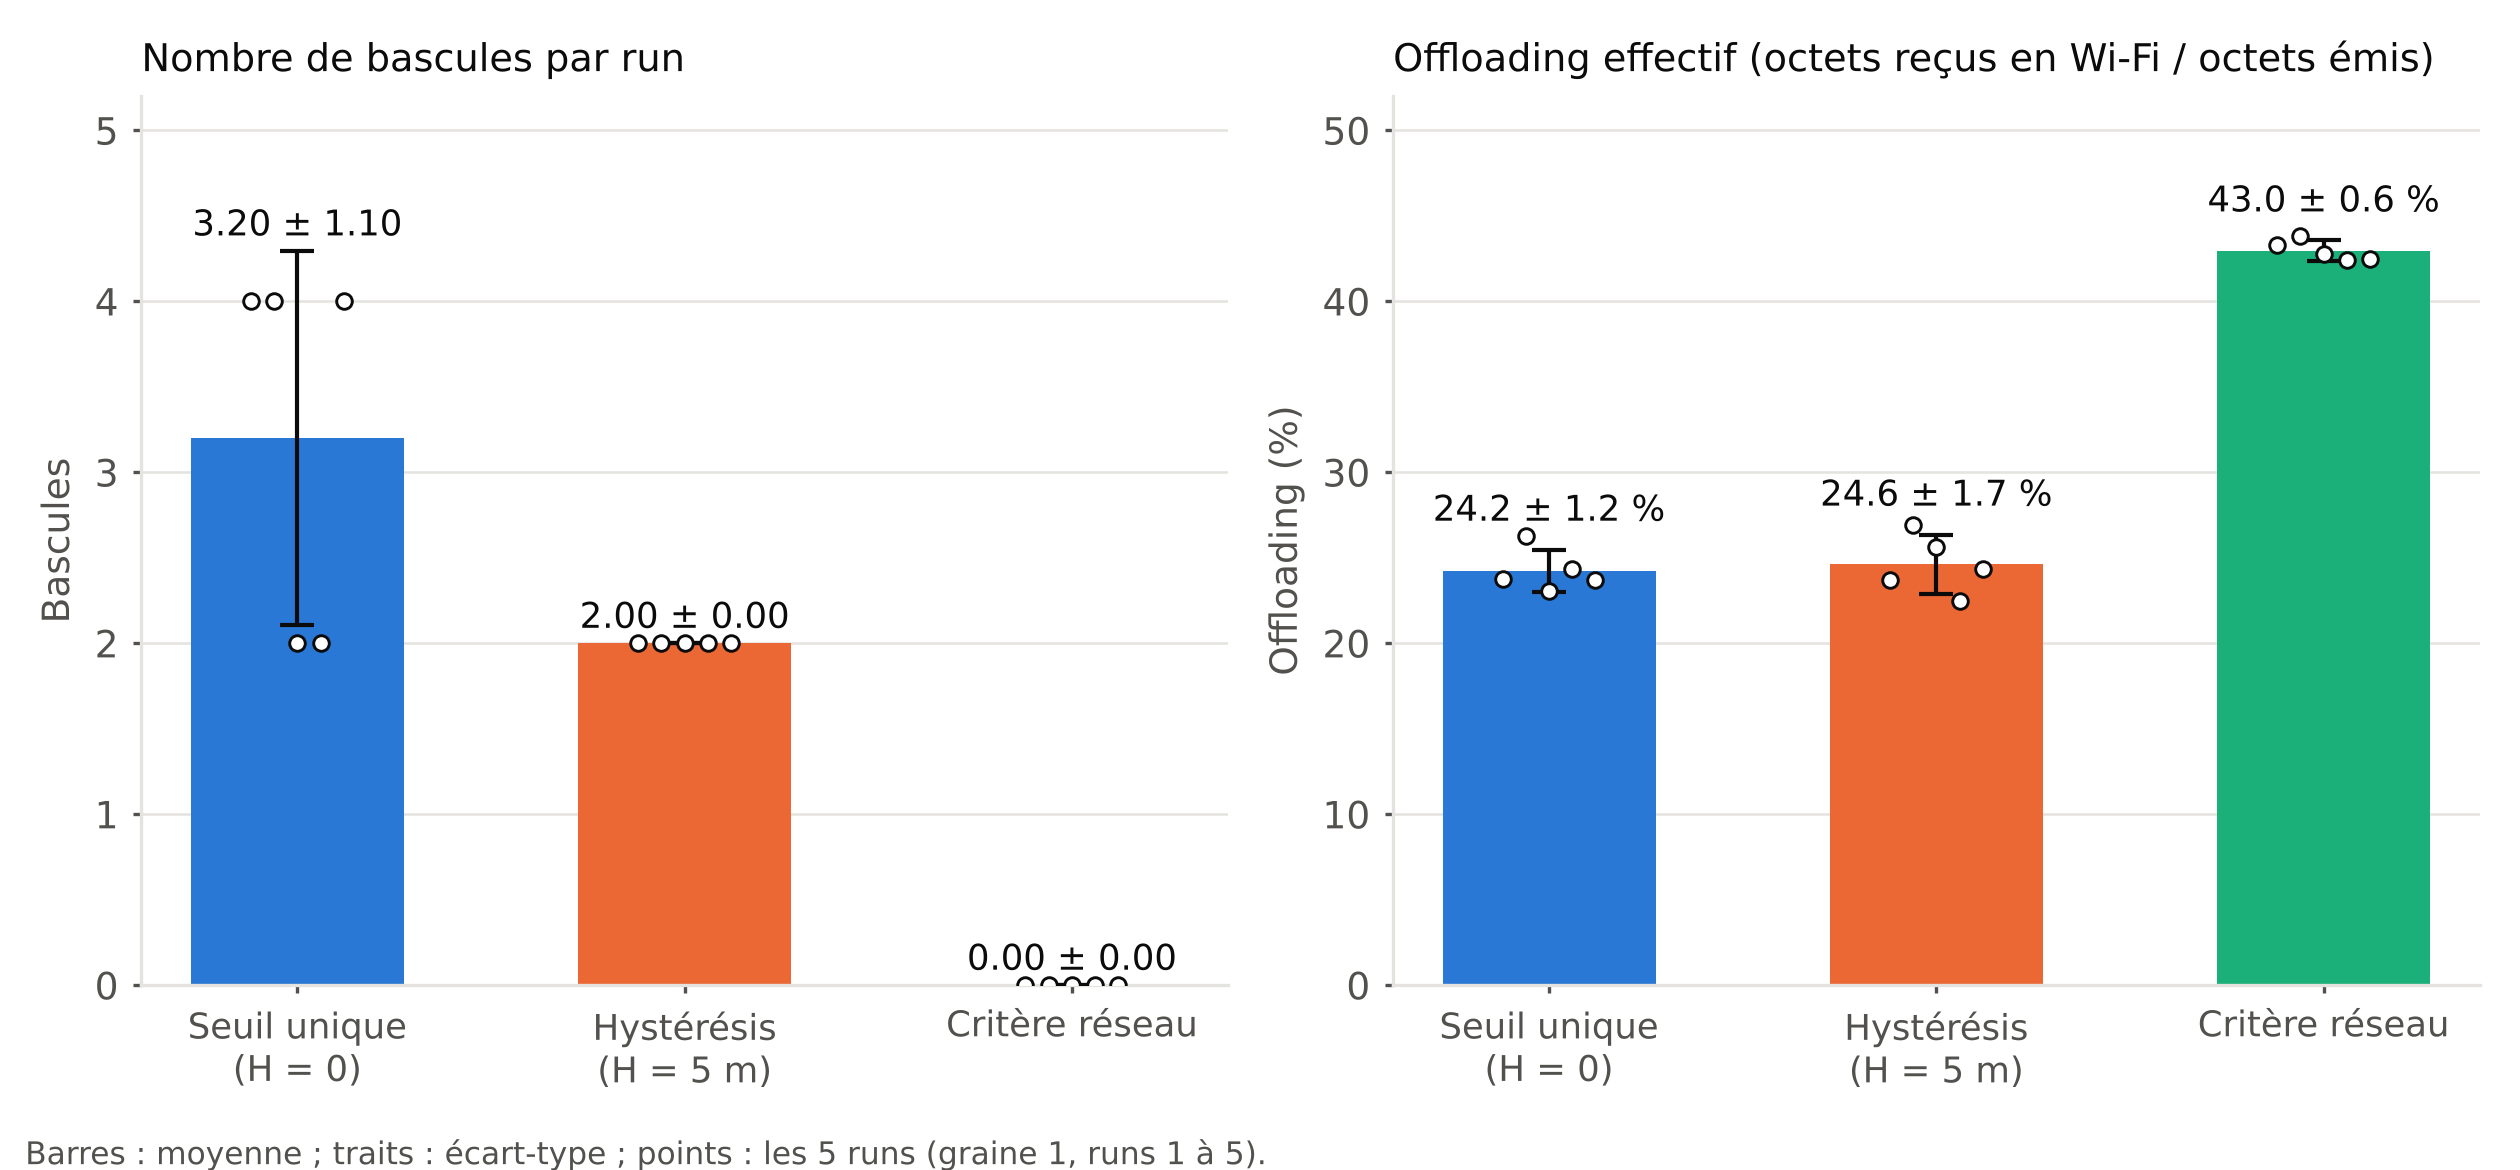
\includegraphics[width=0.7\textwidth]{img/C/pic5_median.png}
      \caption{Nombre de bascules et taux d'offloading par critère (barres + écart-type)}
\end{figure}

\subsection{Analyse}

\paragraph{Nombre de bascules.}
Sans hystérésis, le bruit de mesure de position ($\sigma_d=3$~m) provoque des
bascules supplémentaires lorsque l'UE franchit la frontière du hotspot :
$3{,}20 \pm 1{,}10$ bascules en moyenne, au lieu des deux bascules
attendues (entrée puis sortie). Avec une hystérésis de 5~m, on obtient
exactement deux bascules et aucun ping-pong sur les cinq runs. Ce résultat est
cohérent avec la question B5. Le critère réseau, lui, ne produit aucune
bascule, par construction.

\paragraph{Interruption de service.}
Pour les deux critères terminal, aucune fenêtre de 100~ms n'est passée sous
50\,\% du débit nominal autour des bascules : l'interruption mesurée est nulle.
Seul un pic de délai d'environ 20~ms (contre 13,5~ms en moyenne) est visible.
Ce résultat doit être relativisé : dans NS-3, la bascule se réduit à une
modification de route IP, sans réassociation Wi-Fi ni renégociation d'adresse,
et la résolution de mesure est de 100~ms. Pour le critère réseau, la notion
d'interruption par bascule n'a pas de sens puisqu'il ne bascule jamais en
cours de flux.

\paragraph{Pertes et continuité du service.}
C'est la différence principale entre les approches. Le flux UDP du critère
réseau est « épinglé » sur le Wi-Fi dès t = 1~s. Lorsque l'UE est hors de la
couverture de l'AP, les paquets sont perdus sans qu'aucun mécanisme ne
rebascule le flux vers LTE : on mesure $57{,}04 \pm 0{,}59$\,\% de perte et
44,5~s passées sous le seuil sur 78~s. Les critères terminal, eux, disposent de
LTE comme chemin de repli et n'ont aucune perte. Cette perte provient donc de
l'absence de prise en compte de la mobilité, et non d'un défaut du lien Wi-Fi :
dans l'exécution de contrôle de la question B8, où l'UE reste dans la zone du
hotspot, la perte est nulle.

\paragraph{Taux d'offloading.}
Les critères terminal déchargent environ 24--25\,\% du volume vers le Wi-Fi,
ce qui correspond à la traversée d'une zone de rayon 50~m à 5~m/s. Le critère
réseau atteint environ 43\,\% de volume livré en Wi-Fi : le Wi-Fi reste
utilisable bien au-delà du rayon nominal de 50~m (le déficit de 44,5~s hors
couverture correspond à un rayon effectif de l'ordre de 80~m
Calculé sur les 5 runs par \texttt{rxBytesWifi / (txBytesWifi + txBytesLte)}, il vaut $0{,}43 \pm 0{,}01$.
Le seuil de distance de 50~m est donc conservateur et laisse de la capacité
Wi-Fi inutilisée. En revanche, ce taux plus élevé n'est pas un gain « net » :
il est obtenu au prix de 57\,\% de paquets perdus.

\paragraph{Variabilité entre graines.}
Les écarts-types sont faibles, car la seule source d'aléa est le décalage
latéral $b$ et, pour les critères terminal, le bruit de mesure ; le temps
passé dans le hotspot varie peu avec $b$. Seul le nombre de bascules de
\texttt{dist\_h0} présente une dispersion marquée, ce qui souligne la
sensibilité du seuil unique au bruit de mesure.

\paragraph{Limites de la comparaison.}
\begin{itemize}
  \item Le critère réseau n'a pas de chemin de repli pour le flux UDP, alors
        que les critères terminal en ont un : la comparaison des pertes
        oppose donc deux politiques et pas seulement deux critères.
  \item En mode réseau, un flux TCP supplémentaire circule sur LTE, ce qui n'est
        pas le cas dans les configurations terminal. Le taux d'offloading ne
        porte que sur le flux UDP.
  \item Le shadowing a été désactivé (\texttt{shadowSigma}=0). Lors de nos essais
        avec shadowing activé, aucun paquet n'était livré sur le Wi-Fi ; la
        cause n'a pas été identifiée et la campagne a donc été menée sans
        shadowing.
  \item Cinq graines seulement, sans test statistique inférentiel.
\end{itemize}

\subsection{Quelle approche privilégier ?}

\begin{table}[H]
\centering
\caption{Synthèse comparative des deux familles de critères}
\small
\begin{tabular}{p{3.2cm}p{5.6cm}p{5.6cm}}
\toprule
 & Orienté terminal (distance/RSSI) & Orienté réseau (protocole/débit) \\
\midrule
Mobilité de l'UE & Adapté : suit la couverture réelle et garde LTE en repli & Inadapté pour un UE mobile : aucun suivi de la couverture \\
Nature du trafic & Indifférente à la nature du flux & Exploite le type de flux (UDP débit élevé vs TCP) \\
Stabilité & Risque de ping-pong, atténué par l'hystérésis & Aucune bascule, aucune oscillation \\
Calcul requis & Mesures et décision dans le terminal & Décision centralisée, une fois par flux \\
Information nécessaire & Position ou RSSI de l'UE & Protocole et débit des flux \\
\bottomrule
\end{tabular}
\end{table}

Le critère \textbf{orienté terminal} est préférable lorsque l'UE est mobile ou
lorsque la couverture Wi-Fi est limitée : la décision s'appuie sur l'état
réel du lien et la continuité de service est assurée par LTE. Son coût est un
traitement dans le terminal (mesure et hystérésis) et un risque de bascules
répétées.

Le critère \textbf{orienté réseau} est adapté à des terminaux quasi
statiques ou situés durablement dans la zone Wi-Fi, avec un trafic bien
identifié (par exemple un flux UDP à débit élevé), et lorsque l'opérateur
souhaite centraliser la politique sans solliciter le terminal. Il est
inadapté à un UE mobile tant qu'il n'est pas complété par une réévaluation
périodique du chemin (par exemple à partir du débit mesuré par FlowMonitor),
comme le suggère l'énoncé.

% ---------------------------------------------------------------------
\section{Question 10 : Conclusion sur le Wi-Fi offloading}
% ---------------------------------------------------------------------

Les expériences de la partie B permettent de dégager les conclusions suivantes.

\paragraph{Intérêt pour l'opérateur.}
Lorsque l'UE est dans la zone du hotspot, le Wi-Fi absorbe l'intégralité du
flux UDP de 2~Mb/s, qui n'occupe alors plus les ressources radio LTE. Dans
notre scénario, 24 à 25\,\% du volume est déchargé avec un critère terminal
et jusqu'à environ 43\,\% avec le critère réseau. Il faut toutefois noter
qu'avec un seul UE, nous mesurons une \emph{part du volume} déplacée vers le
Wi-Fi et non une réduction effective de congestion : le gain de charge pour le
réseau LTE n'a pas été quantifié sous charge.

\paragraph{Coût en stabilité.}
Un critère à seuil unique est sensible au bruit de mesure et produit des
bascules supplémentaires ($3{,}2 \pm 1{,}1$ bascules au lieu de 2). L'hystérésis
supprime ce ping-pong, au prix d'une zone de décision plus large qui, si elle
est trop grande, peut empêcher l'accès au Wi-Fi (question B5). Dans la
simulation, les bascules n'entraînent ni perte ni interruption mesurable à la
résolution de 100~ms ; ce résultat ne tient toutefois pas compte de la
réassociation Wi-Fi, de la renégociation IP ou de la rupture éventuelle de
sessions TCP, qui existent dans un réseau réel.

\paragraph{Pertinence du critère de bascule.}
\begin{itemize}
  \item \emph{Distance :} simple à mettre en \oe uvre, mais elle ignore la
        qualité réelle du lien et le seuil nominal sous-exploite la couverture
        effective.
  \item \emph{RSSI :} plus représentatif des conditions radio réelles, avec un
        comportement proche de la distance dans notre canal sans obstacles
        (question B7), mais dont l'intérêt devrait apparaître en milieu urbain
        dense ou en intérieur.
  \item \emph{Protocole/débit décidés côté réseau :} cohérent avec la nature du
        trafic et sans oscillation, mais aveugle à la position de l'UE : il
        provoque 57\,\% de pertes pour un UE mobile qui quitte la couverture.
\end{itemize}

\paragraph{Recommandation.}
Aucun critère isolé n'est satisfaisant pour un terminal mobile. Une approche
combinée est préférable : une politique réseau décide quels flux sont
\emph{éligibles} au Wi-Fi (par protocole et débit), tandis qu'un critère
terminal avec hystérésis, éventuellement fondé sur le RSSI, décide à quel
\emph{moment} utiliser le Wi-Fi, avec LTE comme chemin de repli.

\paragraph{Limites de l'étude.}
Un seul UE et un seul point d'accès, un canal sans shadowing, des bascules
réduites à un changement de route IP, un nombre limité de graines et
l'absence de test statistique inférentiel. Les résultats décrivent le
comportement du scénario simulé et ne se généralisent pas sans campagnes
complémentaires.
